\documentclass[12pt, a4]{report}
\usepackage[utf8]{inputenc}
\usepackage[margin=0.8in]{geometry}
\def\thesection{\arabic{section}}
\setcounter{tocdepth}{4}
\usepackage{graphicx}
\graphicspath{ {images/} }
% Below are for the code blocks
\usepackage{listings}
\usepackage{courier}
\usepackage{verbatim}
\usepackage{color}
\usepackage{rotating}

% Below are table config
\setlength{\arrayrulewidth}{0.5mm}
\setlength{\tabcolsep}{10pt}
\renewcommand{\arraystretch}{1.5}

\definecolor{codegreen}{rgb}{0,0.6,0}
\definecolor{codegray}{rgb}{0.5,0.5,0.5}
\definecolor{codepurple}{rgb}{0.58,0,0.82}
\definecolor{backcolour}{rgb}{0.95,0.5,0.92}
\definecolor{bittersweet}{rgb}{1.0, 0.44, 0.37}
\definecolor{cosmiclatte}{rgb}{0.93, 0.93, 0.93}
\definecolor{eggshell}{rgb}{0.94, 0.94, 0.9}
\definecolor{fandango}{rgb}{0.71, 0.2, 0.54}

\lstdefinestyle{mystyle}{
	backgroundcolor=\color{cosmiclatte},   
	commentstyle=\color{codegreen},
	keywordstyle=\color{fandango}\small,
	numberstyle=\tiny\color{codegray},
	stringstyle=\color{codepurple},
	basicstyle=\ttfamily\footnotesize,
	breakatwhitespace=false,        
	breaklines=true,               
	captionpos=b,                    
	keepspaces=true,  
	numbers=left,                    
	numbersep=5pt,                  
	showspaces=false,                
	showstringspaces=false,
	showtabs=false,                  
	tabsize=2
}

\lstset{style=mystyle}

\title{2810, Software Technologies Assignment 1}
\author{Zaymon Foulds-Cook, s5017391 \textbar{} Natnicha Titiphanpong, s2940970}%\thanks{}}
\date{\today}

\begin{document}

\begin{titlepage}
	\maketitle
\end{titlepage}
 \tableofcontents
\pagebreak
\section{Software Technologies Assignment 1}
\subsection{Problem Statement}
	\par 
	
\subsection{User Requirements}
	\textbf{The following list itemizes the user requirements for the implementation of the Ladder-gram program}
	\begin{itemize}
		\item The user should be able to interact with the program by specifying the start and goal word
		\item The user should be able to select an option to supply a list of words that cannot be used in the path solution
		\item The user should be able to select an option to find the shortest path from start word to goal word
	\end{itemize}
	
\subsection{Software Requirements}
	\textbf{The following list itemizes the software requirements for the implementation of the Ladder-gram program}
	\begin{itemize}
		\item The program will notify the user if the inputs are invalid
		\item The program will notify the user if a solution was found
		\item If a valid solution is found the program will print it to the console
		\item If the user selects the shortest path solution, the program will print the shortest path to the console
		\item If the user chooses to input a list of unusable words, the program will remove those words from the solution's list
		\item The program will report the length of the solution found 
	\end{itemize}
	\pagebreak
	
\subsection{Software Design}
	\subsubsection{High Level Design - Logical Block Diagram}

	\begin{figure}[!h]
	\centering
	\includegraphics[scale=0.6]{Logical_Block_Laddergram}
	\caption{Logical block diagram for the Python implementation of Ladder-gram}
	\end{figure}
				
	\pagebreak

	\subsubsection{Structure Chart - UML}
	\paragraph{}

	\begin{figure}[!h]
	\centering
	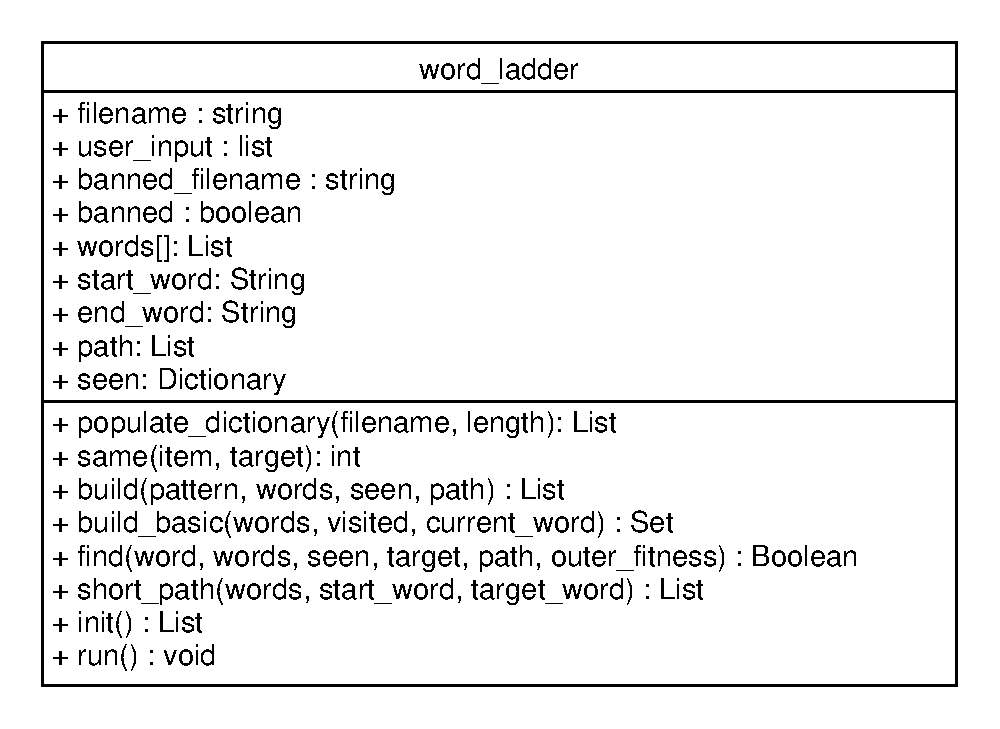
\includegraphics[scale=0.7]{UML}
	\caption{UML diagram for the Python implementation of Ladder-gram}
	\end{figure}


	\subsubsection{List all functions in the software}
	\textbf{	Functions in the Ladder-gram Program}
	\begin{enumerate}
		\item
			\textbf{populate\_dictionary}
			\textbar{}  Function that takes in a filename and a word length and returns a list that contains all words in the file of the specified length.
			\par Input Parameters: filename, length
			\par Side Effects:
			\begin{itemize}
				\item Populate words list
			\end{itemize}
			\par Returns: List
		\item
			\textbf{same}
			\textbar{}  Function that determines how similar two words are by comparing characters in-place. Returns number of characters that are the same.
			\par Input Parameters: str1, str2
			\par Side Effects: None
			\par Returns: integer
		\item
			\textbf{build}
			\textbar{}  Function that returns a list of all words that are one letter away from the last word in the path and have not been seen before.
			    Function also calculates the fitness of each word and adds it with the word in a tuple.
			\par Input Parameters: pattern $($regex pattern$)$, words, seen, path
			\par Side Effects: None
			\par Returns: List of tuples
		\item
			\textbf{find}
			\textbar{}  Recursive function that finds a path from one word two another of the same length by going through intermediary words which are one character different.
			\par Input Parameters:
			\par Side Effects
			\begin{itemize}
				\item `Path' global variable gets modified 
				\item `Seen' global variable gets modified
			\end{itemize}
			\par Returns: Boolean
	\end{enumerate}
	
	\begin{comment}
			\item
				\textbf{}
				\textbar{}  
				\par Input Parameters:
				\par Side Effects
				\begin{itemize}
				\item 
				\end{itemize}
				\par Returns:
	\end{comment}
	
	\subsubsection{List all of the data structures in the Ladder-gram program}
		\par Finish this!
		\begin{enumerate}
				\item
					\textbf{Dictionary}
					\textbar{} Purpose
					\par Used in the following functions:
					\begin{itemize}
						\item find
						\item build
					\end{itemize}
				\item
					\textbf{List}
					\textbar{} Purpose
					\par Used in the following functions:
					\begin{itemize}
						\item find
						\item build
						\item populate\_dictionary
					\end{itemize}
				\item
					\textbf{Tuple}
					\textbar{} Purpose
					\par Used in the following functions:
					\begin{itemize}
						\item find
						\item 
					\end{itemize}
				\item
					\textbf{String}
					\textbar{} Purpose
					\par Used in the following functions:
					\begin{itemize}
						\item find
					\end{itemize}
		\end{enumerate}
	
		
	\subsubsection{Detailed Design}
	
	
	\textbf{Generate Solutions Pseudo-code}
	
	\begin{comment}
			\begin{figure}[h]
			\lstinputlisting[language=Python]{pseudocode_New.py}
			\caption{Psuedo-code for the generate solutions algorithm}
			\end{figure}
	\end{comment}

	
	\pagebreak
	\subsection{Configuration Management and Version Control}
		\par 
		The development of this program required the use of version control software to evenly distribute tasks, as well as monitor the changes through a log. GitHub was designed for users as a way to manage documents, programs and other information. GitHub was neccessary for sharing of files and the ability to compare files and identify differences and merge changes if needed prior to commit. Version control was used to ensure each developer could work on tasks individually as well, even after finishing a formal collaboration. The software records a log of past commits pushed to the respository which alows for backtracking of file versions.
	
	\subsection{Unit Tests}


		\begin{tabular}{ |p{0.5cm}|p{5cm}|p{5cm}|p{5cm}| }
			\hline
			No. & Test Case & Expected Results & Actual Results \\
			\hline
			1.0 & Read in File & & \\
			1.1 & File name does not exist & Exception handled & Exception handled\\
			1.2 &AL & ALB & blank \\
			2.0    &DZ & DZA & blank \\
			2.1 & AS & ASM & blank\\
			3.0 & AD & AND   & blank \\
			3.1 & AO & AGO & blank\\
			\hline
		\end{tabular}
		
	\subsection{Requirement Acceptance Tests}

	\subsection{User Instructions}



	
\end{document}
